\documentclass[../main.tex]{subfiles}

\begin{document}
    A laser (light amplification by stimulated emission of radiation) is a device for the creation and amplification of  coherent light. For this reason, lasers enable us to use light in a highly controlled manner, which is used in communication (light pulses in fibre cables), medicine, spectroscopy research etc.\\ 

    \noindent Generally speaking, a laser has three important components: a pump, an active medium, and a cavity. The active medium is placed inside the cavity (e.g. between two mirrors) and is then excited with the pump. This causes the atoms of the active medium to undergo absorption processes, which in turn enables spontaneous emission to take place.\\

    \noindent If the rate of absorption is higher than the rate of spontaneous emission, a population inversion can take place: more atoms now occupy exited states than atoms occupy the ground state. Photons that are spontaneously emitted have the opportunity to statt oscillating in the cavity (e.g. being reflected back and forth between two mirrors). During this Osillation, the photons can take part in stimulated emission, which is a coherent process and thus produces the feature coherent laser light.\\

    \noindent In case of the Helium Neon laser the active medium is given by a gaseous mixture of Helium and Neon Atoms. The relevant state transitions are depicted in figure \ref{fig:Einleitung-Termschema}. It has to be noted that due to some effects (energy-time-uncertainty, doppler effect), laser lines are not perfectly sharp peaks but are instead broadened. Furthermore the oscillation of the photons inside the cavity is very sensible, small deviations from a perfect cavity setup have notable effects on the laser power, resulting in the loss of lasing in the extreme case.

    \begin{figure}[H]
        \centering
        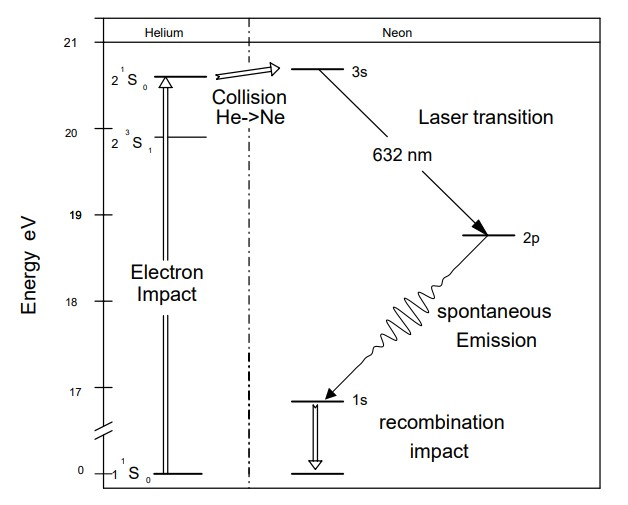
\includegraphics[width=7cm]{Bilddateien/Einleitung/Einleitung-Termschema.jpg}
        \caption{Schematic term diagram for relevant energy levels in the HeNe-laser. For Pumping, electrons are used to excite Helium atoms from the $1S_0$ state (I) into the $2S_0$ state. Through collisions, this energy is used to excite Neon atoms to the $3s$ (II) state. The laser transitions (laser lines) are from this state to the $2p$ (III) state. This is followed by relaxation into the $1s$ (IV) state. Alltogether, the states labelled from (I) to (IV) form a 4-level system, which can achieve a population inversion between lasing states more easily than a 3-level system. Population inversion is not possible with a 2-level system. In reality, states (II) and (III) are degenerate and give rise to many laser transitions of similar wavelength.}
        \label{fig:Einleitung-Termschema}
    \end{figure}

\end{document}